%Preamble
% Some of these are recommended by "9 LaTeX packages everyone should use" http://www.howtotex.com/packages/9-essential-latex-packages-everyone-should-use/, 
%others were added as I came across the need for them.
\RequirePackage[l2tabu, orthodox]{nag} % has to go here in the preamble. Checks for obsolete stuff.
\documentclass{article} % the type of document
\pagestyle{plain}
\usepackage[utf8]{inputenc}
\usepackage[table, usenames, dvipsnames]{xcolor}
\definecolor{lightgray}{gray}{0.9} % I used this for the table background colour
\usepackage{multirow} % needed if cells in a table need to span more than one row
\usepackage{tabu} % makes table columns all have the same width
\usepackage{verbatim}
\usepackage[english]{babel} % so that the document follows the conventions of a  particular language eg english.
\usepackage[documents]{ragged2e}
\usepackage{amsmath} % for maths including align/align*
\usepackage[a4paper]{geometry} % for adjusting page margins
\usepackage[rightcaption]{sidecap}
\usepackage[skip=true,justification=justified,singlelinecheck=false,font=small,format=plain,labelfont=bf,up,textfont=normal,up]{caption}
\usepackage{graphicx} % needed for inserting figures eg \includegraphics
\graphicspath{ {figures/} } %Name of the folder in the project in which all the images are kept.
\usepackage{microtype} % improves spacing and general look of the document.
\usepackage{siunitx} % helps with units and numbers
\usepackage{booktabs} % a way of creating tables without vertical separators. I haven't used this yet, and I don't think it is essential.
\usepackage[
backend=biber,
style=authoryear,
sorting=ynt
]{biblatex} % needed for citations and references
\addbibresource{references.bib} % name of the references file
\usepackage{gensymb} % not sure. Makes some symbols work.
\usepackage{csquotes}
\usepackage{hyperref} % needed for hyperlinks, internal and external. Needs to go at the end of the preamble, except for a few things eg cleveref
\hypersetup{
    colorlinks=true,
    linkcolor=blue,
    filecolor=magenta,      
    urlcolor=cyan,
} % style of the hyperlinks
\urlstyle{same}
\usepackage{cleveref}
%\usepackage{exercise} % does all the things with exercises and solutions.
\usepackage{exsheets} % does all the things with exercises and solutions.
\usepackage{enumitem}

%\\\\\\\\\\\\\\\\\\\\\\\\\\\\\\\\\\\\\\\\\\\\\\\\\\\\\\\\\\\\\\\\\\\\\\\\\\\\\\\\\\\\\\\\\\\\\\\\\\\\\\\\\\\\\\\\\\\\\\\\\\\\\\\\\\\\\\
% Title stuff
\title{Questions on the Solar Resource}
\author{Michael Hunt}
\date{}


\begin{document}
\maketitle

\section*{Exercises}
\begin{question}\label{qu:ex1}
What is meant by the following terms?
    \begin{enumerate}[label=\alph*)]
        \item Solar altitude (also known as sun height)
        \item Solar azimuth angle
        \item Zenith
        \item Zenith Angle
        \item Inclination
        \item Irradiation
        \item Irradiance
        \item Albedo 
        \item Diffuse Radiation
        \item Global Irradiance
        \item Air Mass
    \end{enumerate}
\end{question}
\begin{solution}
    \begin{figure}[h]
    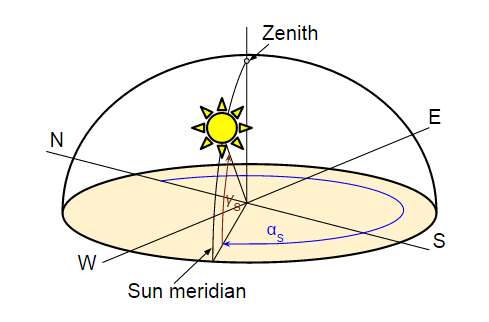
\includegraphics{SolarAngles}
    \caption{The zenith is the direction perpendicularly up from the Earth. $\gamma_S$ is the sun height or solar altitude angle. It tells us how high the Sun is in the sky and is measured from the horizon up to the sun. Its complement is the solar zenith angle $=90-\gamma_S$, which is the angle between the zenith and the sun.  The solar azimuth angle, $\alpha_S$, tells us the direction of the Sun and is measured clockwise from true north. }
    \end{figure}
    \begin{enumerate}[label=\alph*)]
        \item Solar altitude (sun height) measures the height of the sun in the sky. It is the angle between the horizon and the Sun
        \item Solar azimuth angle indicates the direction of the Sun. There are different conventions for this, but that used in these lectures (and in Quaschning \cite{Quaschning2005}, and by \href{http://www.nrel.gov/solar/}{NREL} is that it is the angle measured clockwise from true north to the vertical circle centred on the Earth that goes through the Sun. Thus if the Sun was in the north, the solar azimuth angle would be 0\degree, if in the east, 90\degree, south would be 180\degree and west 270\degree or -90\degree . More generally, the term azimuth angle is used to indicate the direction of something, measure clockwise from true north. If a solar array had an azimuth angle of 180\degree it would be pointing due south, and so on.
        \item The zenith is a line drawn vertically upwards from the Earth
        \item The zenith angle is the angle between the zenith and the Sun's position
        \item Inclination is the angle between the horizontal and a plane eg the plane of a roof
        \item Irradiation is energy received per m$^2$
        \item Irradiance is the power per square metre (eg 1000 W m$^{-2}$)
        \item The albedo of a surface is the fraction of incident radiation that is reflected. This depends on the material, its surface roughness, the angle of incidence and the wavelength of the radiation.
        \item Diffuse Radiation is radiation that has been scattered and hence is travelling along paths which are not directly from the sun.
        \item Global Irradiance is the sum of all radiation falling on a surface (Global = diffuse + direct) 
        \item Air Mass is a unitless measure of the length of the path of light through  the earth's atmosphere in multiples of the thickness of the atmosphere. If the sun is at its zenith, the light passes vertically through the atmosphere and AM is equal to 1. The AM outside the atmosphere is zero.
    \end{enumerate}
\end{solution}

\begin{question}
What is the solar azimuth angle if the Sun is in the following directions:
    \begin{enumerate}
    \item NE
    \item NW
    \item SE
    \item SW
    \end{enumerate}
\end{question}
\begin{solution}
Solar azimuth angles are measure clockwise from true north, so we have
    \begin{enumerate}
    \item NE 45\degree
    \item NW 315\degree
    \item SE 135\degree
    \item SW 225\degree
    \end{enumerate}
\end{solution}

\begin{question}
What value is associated with
    \begin{enumerate}[label=\alph*)]
        \item the solar constant
        \item Peak Sun
        \item 1 peak Sun hour
        \item the "standard solar spectrum"
    \end{enumerate}
\end{question}
\begin{solution}
    \begin{enumerate}[label=\alph*)]
        \item the solar constant = 1360 W m$^{-2}$
        \item peak Sun = 1000 W m$^{-2}$
        \item 1 peak Sun hour = 1000 W m$^{-2}$ for 1 h = 1 kWh of irradiation m$^{-2}$
        \item the "standard solar spectrum" is what you get from a source at 5500 K (the Sun, more or less) seen through AM1.5.
    \end{enumerate}
\end{solution}

\begin{question}
What is the Zenith angle for Cornwall at midday on:
    \begin{enumerate}[label=\alph*)]
        \item the spring equinox
        \item the summer solstice
        \item the autumn equinox
        \item the winter solstice
    \end{enumerate}
\end{question}
\begin{solution}
    \begin{enumerate}[label=\alph*)]
        \item the spring equinox: Zenith Angle = latitude = 50\degree
        \item the summer solstice: Zenith Angle = latitude - 23.5\degree = 26.5\degree
        \item the autumn equinox: Zenith Angle = latitude = 50\degree
        \item the winter solstice: Zenith Angle = latitude + 23.5\degree = 73.5\degree
    \end{enumerate}
\end{solution}

\begin{question}
What is the solar altitude angle for Cornwall at midday on:
    \begin{enumerate}[label=\alph*)]
        \item the spring equinox
        \item the summer solstice
        \item the autumn equinox
        \item the winter solstice
    \end{enumerate}
\end{question}
\begin{solution}
Altitude angle = 90\degree - Zenith angle, so we get
    \begin{enumerate}[label=\alph*)]
        \item the spring equinox: altitude angle = 90 - 50 = 40\degree
        \item the summer solstice: altitude angle = 90 - 26.5 = 63.5\degree
        \item the autumn equinox: altitude angle = 90 - 50 = 40\degree
        \item the winter solstice: altitude angle = 90 -  73.5 = 16.5\degree
    \end{enumerate}
\end{solution}

\begin{question}
What is the ideal inclination for a solar collector in Cornwall at midday on:
    \begin{enumerate}[label=\alph*)]
        \item the spring equinox
        \item the summer solstice
        \item the autumn equinox
        \item the winter solstice
    \end{enumerate}
\end{question}
\begin{solution}
Ideal inclination for solar collection = 90 - solar altitude angle = Zenith angle, giving:
    \begin{enumerate}[label=\alph*)]
        \item the spring equinox: 50\degree
        \item the summer solstice: 26.5\degree
        \item the autumn equinox: 50\degree
        \item the winter solstice: 73.5\degree
    \end{enumerate}
\end{solution}

\begin{question}
    What is the approximate value of the average daily irradiance for Cornwall in:
    \begin{enumerate}[label=\alph*)]
        \item spring
        \item summer
        \item autumn
        \item winter
    \end{enumerate}
\end{question}
\begin{solution}
    \begin{enumerate}[label=\alph*)]
        \item spring \approx 3\ \mathrm{kWh\ day$^{-1}$}
        \item summer \approx 5.5\ \mathrm{kWh\ day$^{-1}$}
        \item autumn \approx 3\ \mathrm{kWh\ day$^{-1}$}
        \item winter \approx 1\ \mathrm{kWh\ day$^{-1}$}
    \end{enumerate}
\end{solution}

\begin{question}
What is the approximate annual irradiance in
    \begin{enumerate}[label=\alph*)]
        \item Cornwall
        \item Scotland
        \item Tunisia
    \end{enumerate}
\end{question}
\begin{solution}
    \begin{enumerate}[label=\alph*)]
        \item Cornwall \approx 1200\ \mathrm{kWh\ y$^{-1}$}
        \item Scotland \approx 900\ \mathrm{kWh\ y$^{-1}$}
        \item Tunisia \approx 2000\ \mathrm{kWh\ y$^{-1}$}
    \end{enumerate}
\end{solution}
\printbibliography
\section*{Solutions}
\printsolutions
\end{document}
